\documentclass{scrartcl}
\usepackage[utf8]{inputenc}
\usepackage{tikz}
\usetikzlibrary{arrows,decorations.pathmorphing,backgrounds,fit,positioning,shapes.symbols,chains,shapes.geometric,shapes.arrows,calc}

\begin{document}

      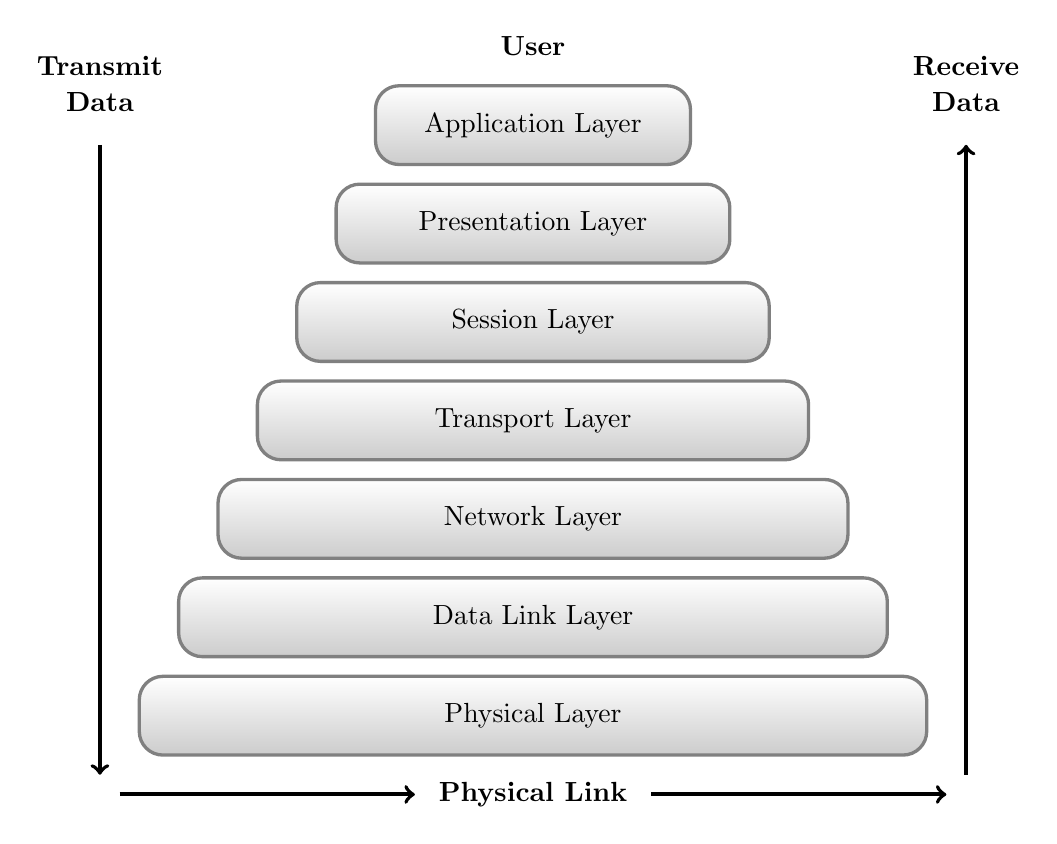
\begin{tikzpicture}
    
        \draw[rounded corners=3mm,very thick,draw=black!50,top color=white,bottom color=black!20] (-2,0) rectangle (2,-1);
        \draw[rounded corners=3mm,very thick,draw=black!50,top color=white,bottom color=black!20] (-2.5,-1.25) rectangle (2.5,-2.25);
        \draw[rounded corners=3mm,very thick,draw=black!50,top color=white,bottom color=black!20] (-3,-2.5) rectangle (3,-3.5);
        \draw[rounded corners=3mm,very thick,draw=black!50,top color=white,bottom color=black!20] (-3.5,-3.75) rectangle (3.5,-4.75);
        \draw[rounded corners=3mm,very thick,draw=black!50,top color=white,bottom color=black!20] (-4,-5) rectangle (4,-6);
        \draw[rounded corners=3mm,very thick,draw=black!50,top color=white,bottom color=black!20] (-4.5,-6.25) rectangle (4.5,-7.25);
        \draw[rounded corners=3mm,very thick,draw=black!50,top color=white,bottom color=black!20] (-5,-7.5) rectangle (5,-8.5);
    
        \node[] at (0, -0.5) {Application Layer};
        \node[] at (0, -1.75) {Presentation Layer};
        \node[] at (0, -3) {Session Layer};
        \node[] at (0, -4.25) {Transport Layer};
        \node[] at (0, -5.5) {Network Layer};
        \node[] at (0, -6.75) {Data Link Layer};
        \node[] at (0, -8) {Physical Layer};
    
        \node[] at (0, 0.5) {\textbf{User}};
        
        \node[] at (-5.5, 0.25) {\textbf{Transmit}};
        \node[] at (-5.5, -0.2) {\textbf{Data}};
       
        \node[] at (5.5, 0.25) {\textbf{Receive}};
        \node[] at (5.5, -0.2) {\textbf{Data}};
       
        \node[] at (0, -9) {\textbf{Physical Link}};    
    
        \draw[->, line width=0.5mm] (-5.5,-0.75) -- (-5.5,-8.75) ;        
        \draw[->, line width=0.5mm] (-5.25,-9) -- (-1.5,-9) ;
        \draw[->, line width=0.5mm] (1.5,-9) -- (5.25,-9) ;
        \draw[->, line width=0.5mm] (5.5,-8.75) -- (5.5,-0.75) ;
        
    \end{tikzpicture}

 \end{document}
